\subsection{Mallado}

\noindent
\justify

Gran parte del \'exito de las simulaciones num\'ericas recaen en la discretizaci\'on del dominio y en la calidad de los elementos que la componen. Se desarroll\'o una metodolog\'ia de mallado autom\'atico a trav\'es de la librer\'ia \textit{Pygmsh} (basada en Python); la cual toma como variables de entrada las dimensiones de la geometr\'ia definida en la secci\'on \ref{geo}. Esta metodolog\'ia emplea elementos de diferentes rangos de tama\~no de malla, como se puede apreciar en la Figura \ref{rango}.

\begin{figure}[h!]
	\centering
	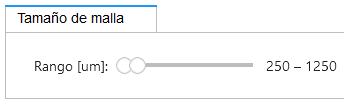
\includegraphics[width=0.5\textwidth]{Images/CFDEM/size.PNG}
	\caption{Rango de tama\~no de malla.}
	\label{rango}
\end{figure}

\noindent
\justify

El algoritmo ejecuta, adem\'as, un refinamiento autom\'atico en la zona en donde ocurre el mayor grado de sedimentaci\'on: en la superficie inclinada, como se aprecia en la Figura \ref{malla:geo}.

\begin{figure}[h!]
	\centering
	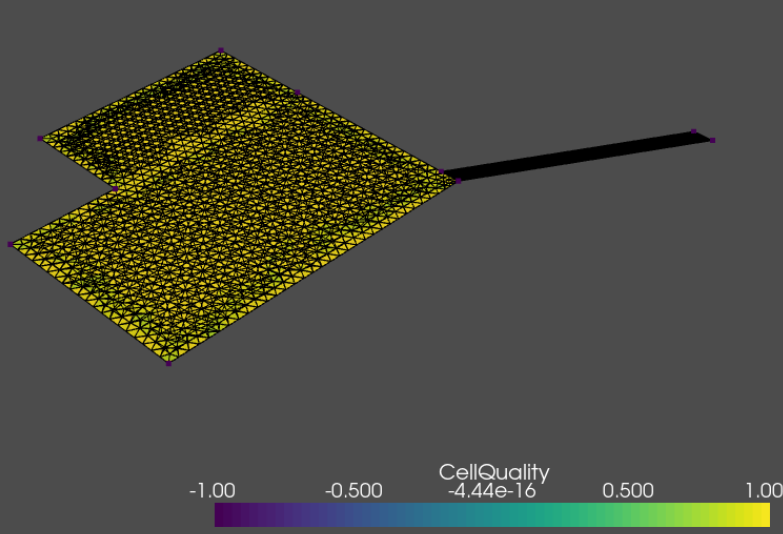
\includegraphics[width=\textwidth]{Images/CFDEM/malla.PNG}
	\caption{Mallado de la geometr\'ia.}
	\label{malla:geo}
\end{figure}

\noindent
\justify

De manera resumida, la malla desarrollada presenta los siguientes datos:

\begin{table}[h!]
	\centering
	\begin{tabular}{|c|c|}
		\hline
		\textbf{Par\'ametro} & \textbf{Valor} \\ \hline
		Tipo de malla & Tetrah\'edrica \\ \hline
		N\'umero de elementos & 12429 \\ \hline
		N\'umero de nodos & 5894 \\ \hline	
	\end{tabular}
	\caption{Datos de la malla generada.}
	\label{malla}
\end{table}